\documentclass[11pt, a4paper]{article}
\usepackage{amsmath, amsthm, amssymb, calrsfs, wasysym, verbatim, bbm, color, graphics, geometry}
\usepackage[utf8]{inputenc} % comment when using lualatex
%\usepackage[italian]{babel} % lingua e a-capo-sillabato
\usepackage{fullpage}
\usepackage{graphicx}
%\usepackage[hidelinks]{hyperref,xcolor} % link di pagina
\usepackage[bottom]{footmisc} % note appiccicate al fondo della pagina
\usepackage{float} % per posizionamento immagini
\usepackage{cancel}

\geometry{tmargin=.75in, bmargin=.75in, lmargin=.75in, rmargin = .75in}  

\newcommand{\R}{\mathbb{R}}
\newcommand{\C}{\mathbb{C}}
\newcommand{\Z}{\mathbb{Z}}
\newcommand{\N}{\mathbb{N}}
\newcommand{\Q}{\mathbb{Q}}
\newcommand{\M}{\mathbb{M}}
\newcommand{\Cdot}{\boldsymbol{\cdot}}

\newtheorem{thm}{Theorem}
\newtheorem{defn}{Definition}
\newtheorem{conv}{Convention}
\newtheorem{rem}{Remark}
\newtheorem{lem}{Lemma}
\newtheorem{cor}{Corollary}



\definecolor{dkgreen}{rgb}{0,0.6,0}
\definecolor{gray}{rgb}{0.5,0.5,0.5}
\definecolor{mauve}{rgb}{0.58,0,0.82}


\title{Cryptography Notes }
\author{Raffaele Castagna}

\date{Academic Year 2025-2026}

\begin{document}

\maketitle
\tableofcontents
\newpage

\section{Intro to Cryptography}
\label{Intro}
\subsection{Secure Communication}
We have multiple goals in cryptography, the most important ones being:
\begin{center}
    \textbf{Confidential Integrity}
    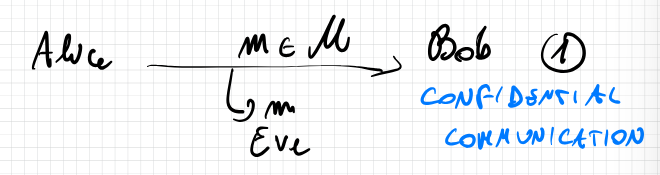
\includegraphics{img/CF comm.png}
\end{center}
\begin{center}
    \textbf{Message Integrity}
    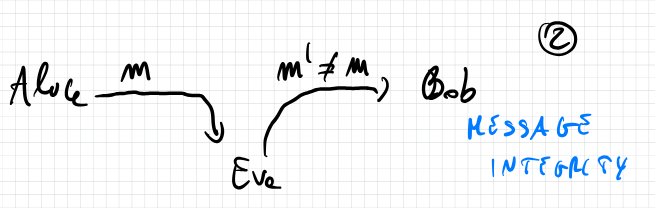
\includegraphics{img/Msg int.png}
\end{center}
Basically we want our message to be both \textbf{confidential}, so no-one except the intended target sees it and we it to be unmodified, so that its \textbf{integrity} has not been compromised.\\\\
There are many different ways to do this, but in our case we only see two major ways:
\begin{itemize}
    \item \textbf{Symmetric Cryptography}:  $\text{Where Alice and Bob share a key } k \in \mathcal{K} \text{,the key is random and unknown to Eve}$
    \item \textbf{Assymetric Cryptography}: Where Alice and Bob do not share a key, but they have each their own key pair $(p_k,s_k)$ where $p_k$ is the public key and $s_k$ is the secret/private key
\end{itemize}

\subsection{Unconditional Security}
To achieve confidential communication, we use symmetric cryptography.
\begin{center}
    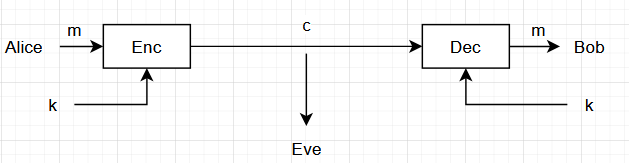
\includegraphics{img/US.png}
\end{center}
With $m \in \mathcal{M}, c \in \mathcal{C}, k \in \mathcal{K}$\\\\
In this case we have Alice sending a message \textit{m} which is then encrypted utilizing a randomly generate key \textit{k} to generate the cyphertext \textit{c}, after that to get back to the initial message \textit{m}, Bob will then need to decrypt it utilizing his own key \textit{k} on cyphertext \textit{c}.\\
In a more formal way we can define Symmetric encryption (SKE) as $\prod = (Enc, Dec)$ such that:
\begin{itemize}
    \item Enc : $\mathcal{M} \times \mathcal{K} \rightarrow \mathcal{C}$
    \item Dec: $\mathcal{C} \times \mathcal{K} \rightarrow \mathcal{C}$
    \item k is uniform over $\mathcal{K}$ (k is chosen according to some distribution)
\end{itemize}
An encryption scheme must satisfy the correctness requirement:
\begin{defn}
    $\forall k \in \mathcal{K}, \forall m \in \mathcal{M} \text{ it holds that } Dec(k,Enc(k,m)) = m$
\end{defn}

\textbf{Kerchoff's Principle}:
\begin{defn}
    Security should not depend on the secrecy of the algorithm but on the secrecy of the key.
\end{defn}
\subsection{Perfect Secrecy}
\begin{defn}
Let M be any distribution over $\mathcal{M}$ and K be uniform over $\mathcal{K}$ (Then observe C = Enc(K,M) in a distribution over C), we say that (Enc,Dec) = $\prod$ is \textbf{perfectly secret}
if $\forall M, \forall m \in \mathcal{M}, \forall c \in \mathcal{C}: Pr[M=m] = Pr(M=m | C=c)$ (The probability that M is m is equal to the probability that M is m knowing that C is c, so by knowing the cyphertext, we dont gain additional information).
\begin{lem}
The following are equivalent:
\begin{itemize}
    \item Perfect Secrecy
    \item M and C are independant
    \item $\forall m,m' \in \mathcal{M}, \forall c \in \mathcal{C}: Pr[Enc(k,m) = c] = Pr[Enc(k,m') = c] \text{ with k being uniform over } \mathcal{K}$
\end{itemize}
\end{lem}
\end{defn}
\subsection{OTP}
Let us see if OTP (\textit{One Time Pad}) is perfectly secret\\
We know that the OTP uses $\oplus$ to generate and later decypher the cyphertext, we have that $K=M=C=\{0,1\}^N$ with N being the length of the string, we know that:
\begin{itemize}
    \item Enc (k,m) = $k \oplus m$
    \item Dec (k,c) = $c \oplus k$ = $(k \oplus m) \oplus k = m$
\end{itemize}
To prove that it is perfectly secret let us utilize the third lemma:
\begin{center}
    $Pr[C=c | M=m'] = Pr[\text{Enc}_k (m') = c] = Pr[m' \oplus K = c] = Pr[K = m' \oplus c] = 2^{-N}$
\end{center}
and therefore:\\
\begin{center}
    $Pr[Enc(k,m') = c] = 2^{-N}$
\end{center}
There seem to be some limitations, the key can only be used once and it must as long as the message,lets assume we encrypt m'' and m':
$c_1 = k \oplus m_1\text{    } c_2 = k \oplus m_2 \text{ therefore } c_1 \oplus c_2 = m_1 \oplus m_2$, so if I know a pair $(m_1,c_1) \text{ then I could compute } m_2$, therefore we cannot encrypt two messages with the same key.
\begin{thm}[Shannon]
Let $\prod$ be any perfectly secret SKE then we have $|\mathcal{K}| \ge |\mathcal{M}|$.
\end{thm}
\begin{proof}
Take $\prod$ to be uniform over $\mathcal{M}$. Take any c s.t. Pr[C=c] $>$ 0.\\
Consider $\mathcal{M'} = \{Dec(k,c): k \in \mathcal{K}\}$ and assume $|\mathcal{K}| < |\mathcal{M}|$ by contraddiction, then:\\
\begin{center}
    $|\mathcal{M}|' \leq |\mathcal{K}| < |\mathcal{M}| \rightarrow |\mathcal{M'}| < |\mathcal{M}| \rightarrow \exists m \in \mathcal{M} \setminus \mathcal{M'}$
\end{center}
Now:\\
\begin{center}
   $ Pr[M=m] = |\mathcal{M}|^{-1} \text{ but } Pr[M=m | C=c] = 0 $
\end{center}

\end{proof}

\subsection{Proof that the lemmas imply eachother}
Let us prove that $1 \implies 2 \implies 3 \implies 1$\\\\
Let us start by proving that $1\implies2$:
\begin{proof}
We know that $Pr[M=m] = Pr[M=m|C=c] \rightarrow \frac{Pr[M=m \wedge C=c]}{Pr[C=c]} = Pr[M=m \wedge C=c] \\= Pr[M=m] * Pr[C = c]$
and therefore we have proved their independence, so $I(M;C) = 0$
\end{proof}
Let us prove that $2 \implies 3$
\begin{proof}
Let us fix an m from M and c from C:\\
$Pr[Enc(K,m) = c] = Pr[Enc(K,M) = c | M = m] \implies Pr[C = c | M = m] = Pr[C=c]$ \\Remember that Enc(...) is c!\\\\ We do the same thing for $m'$ and we get: 
$Pr[C=c | M=m] = Pr[C=c]$ for both of them.\\
Therefore: $Pr[Enc(K,m')= c] = Pr[C=c]$
\end{proof}

And now $3 \implies 1$:
Take any c from C:\\
$Pr[C=c] = Pr[C=c|M=m]$ by 2 (we are claiming this)\\\\
If the claim is true then:\\
$Pr[M=m|C=c] * Pr[C=c] = Pr[M=m \wedge C=c] = Pr[C = c | M = m] * Pr[M=m] \implies$\\\\
\begin{center}
   $\implies$ $Pr[M=m] = \frac{Pr[M=m | C=c] * \cancel{Pr[C=c]}}{\cancel{Pr[C=c|M=m]}}$

\end{center}
However we still need to prove the claim:\\
$$Pr[C=c] = \sum_{m'}^{}Pr[C=c \wedge M=m'] = \sum_{m'}^{}Pr[C=c | M=m'] * Pr[M=m'] =$$\\ $$\sum_{m'}^{}Pr[Enc(K,m') = c | M=m'] * Pr[M=m']\\= \sum_{m'}^{}Pr[Enc(K,m') = c] * Pr[M=m'] $$\\
$$ \sum_{m'}^{}Pr[Enc(k,m) = c] * Pr[M=m'] = Pr[Enc(k,m) = c] * \sum_{m'}^{}Pr[M=m'] \impliedby 1$$\\
$$ Pr[Enc(k,m) = c] = Pr[Enc(K,M) = c | M=m] \rightarrow Pr[C=c | M=m]$$
\subsection{Message Authentication Codes}
\begin{center}
    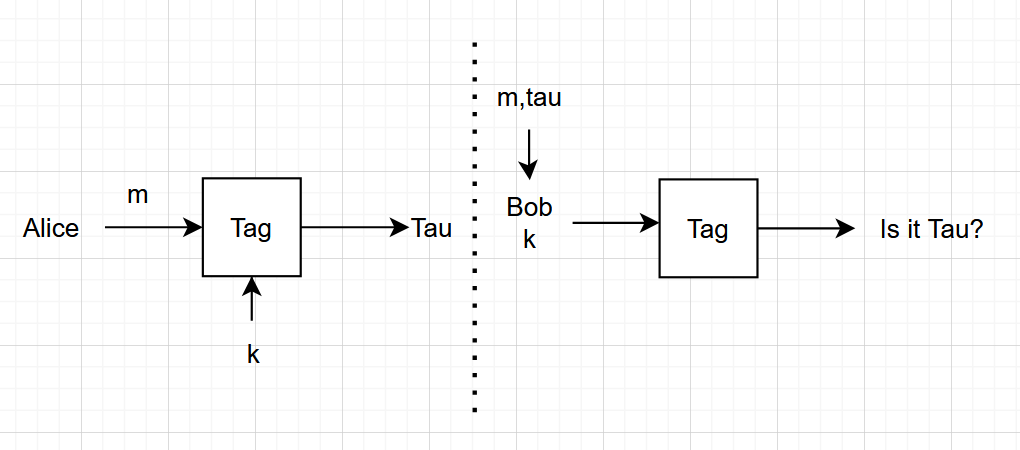
\includegraphics[scale=0.5]{img/MAC.png}
\end{center}
In case it is $\tau$ then we accept it, else no.\\
There is no need to prove correctness as $\tau$ is deterministic, so if we had the same k and m, we should get the same $\tau$\\\\
\textbf{Unforgeability}\\\\
It should be hard to forge $\tau'$ such on msg m' and it should be hard to produce (m,$\tau$) as long as m' $\neq$ m\\
\begin{defn}
\textbf{Statistical secure MAC} We say that $\prod$ = Tag has $\epsilon$-statistical security (unforgeability) if  $\text{ }\forall m,m'\text{ } \in \mathcal{M} \text{ with } m \neq m'\text{ } \forall \tau,\tau' \in \mathcal{T}$:\\
$$Pr[Tag(K,m') = \tau'\text{ } | \text{ }Tag(K,m)= \tau] \leq \epsilon$$
\end{defn}
\textbf{TLDR}: Fix \underline{any} m,m' with m' $\neq$ m take $\tau,\tau'$ on the condition that $\tau$ is tag of m and given $\tau'$, it is always less than or equal to $\epsilon$\\
Here $\epsilon$ is a parameter e.g. $2^{-80}$\\
\textbf{Exercise} Let us prove that it is impossible to get $\epsilon = 0$\\
Because a random $\tau' \in \mathcal{T}$ has probability $\geq \frac{1}{|\mathcal{T}|}$ to be correct it is impossible.\\\\
Note that the definition is valid for One-Time!\\
We will show:
\begin{itemize}
    \item The notion is Achievable
    \item It's inefficient, in fact:
\end{itemize}
\begin{thm}
    Any t-time $2^{-\lambda}$ statistically secure Tag has a key of some (t+1)*$\lambda$
\end{thm}
We will now show that any form of hash function with a particular property satisfies the definition.\\
\begin{defn}
    \textbf{Pairwise independence} A family $\mathcal{H} = \{h_k: \mathcal{M} \rightarrow \mathcal{T}\}_{k \in \mathcal{K}}$ is pairwise independant if: $\forall m,m' \in \mathcal{M} \text{s.t.} m \neq m'$ then:
    $(h(K,m),h(K,m'))$ is uniform over $\mathcal{T}^2 = \mathcal{T} \times \mathcal{T}$ for K uniform over $\mathcal{K}$
\end{defn}

\begin{thm}
    Any family $\mathcal{H}$ of pairwise independent functions directly gives a $\epsilon = \frac{1}{|\mathcal{T}|}-\text{statistically}$ secure MAC.
\end{thm}
\begin{proof}
    Fix any $m \in \mathcal{M}, \tau \in \mathcal{T}$:\\
    $$Pr[Tag(K,m) = \tau] =$$ \\$$ Pr_k[h(K,m)= \tau] = \frac{1}{|\mathcal{T}|}\text{ by pairwise independence}$$\\
    Similiarly, for any m,m' s.t. m $\neq$ m', $\tau,\tau' \in \mathcal{T}$.
    $$Pr_k[Tag(K,m)= \tau \wedge Tag(K,m') = \tau'] =$$
    $$Pr_k[h(K,m)=\tau \wedge h(K,m')= \tau'] = \frac{1}{|\mathcal{T}|^2}$$
    By Bayes:
    $$Pr[Tag(K,m')= \tau' | Tag(K,m) = \tau] = $$
    $$\frac{Pr[h(K,m;) = \tau' \wedge h(K,m) = \tau]}{Pr[h(K,m) = \tau]} =$$
    $$\frac{\frac{1}{|\mathcal{T}|^2}}{\frac{1}{|\mathcal{T}|}} = \frac{1}{|\mathcal{T}|}$$

\end{proof}
Now we need to instantiate it, here is a construction, Let p be a prime:\\
    $$h_{a,b}(m) = am+b \mod p $$
    $$k = (a,b) \in \Z_{p}^2 = \mathcal{K}$$
    $$\Z_p = \mathcal{M} =\mathcal{T}$$
\begin{lem}
    The above $\mathcal{H}$ is \textit{pairwise independant}.
\end{lem}
\begin{proof}
    For all $m,m' \in \Z_p , \tau,\tau' \in \Z_p$ with $m \neq m'$\\
    $$\Pr_{(a,b) \in \Z_{p}^2}[h_{a,b}(m) = \tau \wedge h_{a,b}(m') = \tau'] =$$
    $$\Pr_{(a,b) \in \Z_{p}^2}\left[
        \begin{pmatrix}
        m & 1 \\ m' & 1
        \end{pmatrix}
        \begin{pmatrix}
            a \\ b
        \end{pmatrix} =
        \begin{matrix}
            \tau \\ \tau'
        \end{matrix}\right] = $$ 
        $$\Pr_{(a,b) \in \Z_{p}^2}\left[
        \begin{pmatrix}
            a \\ b
        \end{pmatrix} =
        \begin{pmatrix}
        m & 1 \\ m' & 1
        \end{pmatrix}
        \begin{matrix}
            \tau \\ \tau'
        \end{matrix}\right] = $$
        $$\frac{1}{p^2} = \frac{1}{|\Z_{p}|^2} = \frac{1}{|\mathcal{T}|^2}$$
\end{proof}
\subsection{Randomness Extraction}
Alice and Bob need a \textbf{random} key, how can they generate it?\\
Randomness is crucial for crypto, and two components are necessary in any RNG (e.g. Fortuna, /dev/rand):\\
\begin{itemize}
    \item Randomness extraction: By measuring physical quantities we can get an \textbf{unpredictable} sequence of bits (Not necessarily uniform or for cheap!)\\ From this we extract a \textbf{random} Y which is short (e.g. 256 bits)
    \item Expand it to any amount (polynomial) using a psedorandom generator (PRG) - but this requires computational assumptions.
\end{itemize}
We want to understand how to extract from an unpredictable source X.\\
\textbf{Example \textit{Von Neumann Extractor}}
Assume $B \in {0,1} \text{ s.t. } \Pr[B=0] = p < \frac{1}{2}$.
\begin{itemize}
    \item Sample $b_1 \in B, b_2 \in B$
    \item if $b_1 = b_2$ then Resample
    \item Else output 1 $\iff b_1 = 0, b_2 = 1, \text{ or 0 if } b_1 = 1, b_2 =0$
\end{itemize}
Assuming it outputs something, this will be s.t.\\
$$\Pr[\text{Output 0}] = Pr[\text{Output 1}] = p*(1-p)$$
$$\Pr[\text{No output after N tries}] = (1-2p(1-p))^N \text{ which becomes small for large enough N}$$
We want to generalize this question, ideally we want to design a function Ext that takes a random variable X and outputs an uniform Ext(X), but this is impossible as the source must be unpredictable and Ext is deterministic
\begin{defn}[Min-Entropy]
    The min-entropy of X is: $H_{\infty} = - \log_2\max{\Pr[X=x]}$
\end{defn}
\textbf{Example}:
Let $X \equiv U_m$ Uniform over $\{0,1\}^{N}$. $ H_{\infty} (X) = N$\\
If X is a costant we have $H_\infty (X)$ = 0
\\\\
Here's the next best thing:\\
Design Ext that extracts UNIFORM $Y=Ext(X)$ for every X s.t. $H_\infty (X) \geq k$\\
But this is also impossible, even if $$Ext(X)= b \in \{0,1\}$$ $$k = n-1$$ $$x \in \{0,1\}^n$$\\
And here's why: fix any Ext:$\{0,1\}^n \rightarrow {0,1}$ and let $b \in {0,1}$ be the output of maximing $|Ext^{-1}(b)|$\\
\begin{center}
    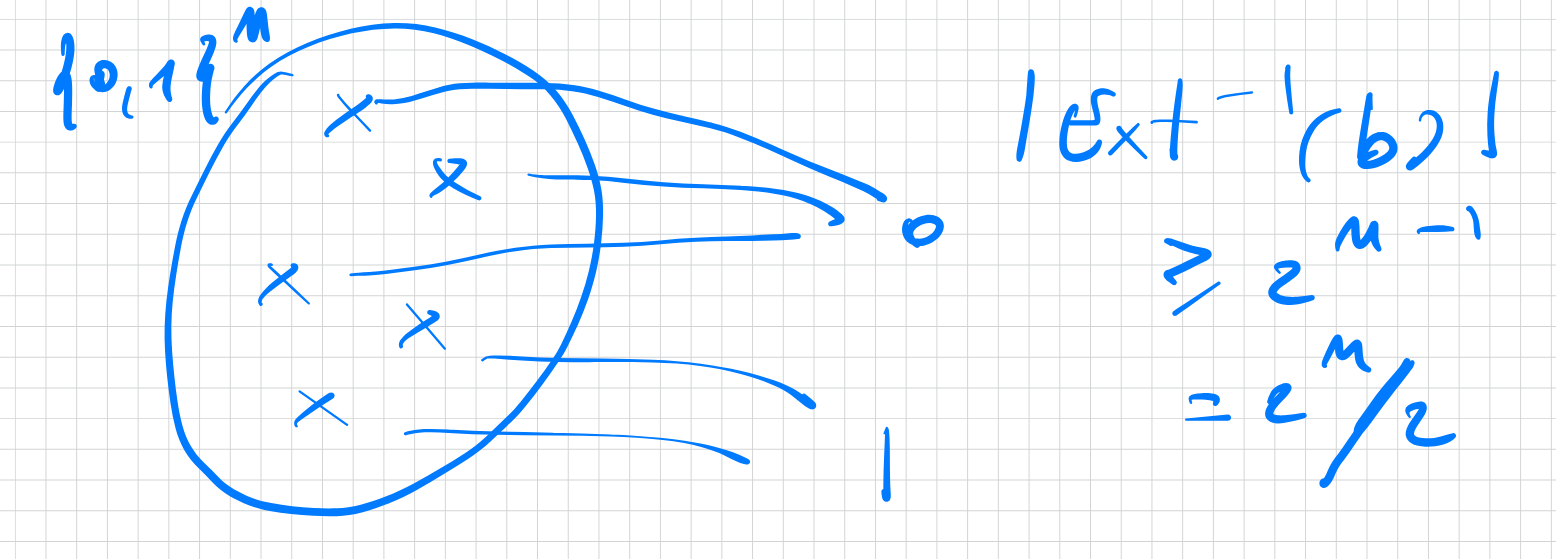
\includegraphics[scale=0.3]{img/expl.png}
\end{center}
The bad X: Define X to be Uniform over $Ext^{-1}(b)$. Since it is uniform: $H_\infty(X) \geq n-1$ but $Ext(X) = b$ so not uniform.\\\\
Solution: Swap the quantifiers.
\begin{defn}[Seeded Extractor]
    A function $Ext: \{0,1\}^n \times \{0,1\}^d \rightarrow \{0,1\}$ is a (k,$\epsilon$)-seeded extractor if for every X over s.t. $H_\infty(X) \geq k$: $$(S,Ext(S,X)) \approx_\epsilon (S,U_e)$$
    for $S \equiv U_d$ (uniform over $\{0,1\}^d$). (Note that $(S,U_e) \equiv U_{d+e}$).
\end{defn}
What does this mean? Thre is a standard way to measure distance between distributionsL
$$ Z \equiv_\epsilon Z' \iff SD(Z,Z') \leq \epsilon$$
$$ SD(Z,Z') = \frac{1}{2} \sum_{z} |Pr[Z=z] - Pr[Z'=z]|$$
This is equivalent: $\forall$ Unbounded adversary A:
$$|Pr[A(z)=1 : z \in Z] - Pr[A(z)=1 : z \in Z']| \leq \epsilon$$
\begin{thm}[Leftover Hash Lemma]
    Let $\mathcal{H} = \{h_s: \{0,1\}^n \rightarrow \{0,1\}^l\}_{s \in \{0,1\}^d}$ be a family of pairwise independent hash functions. Then Ext(x,s) = $h_s(x)$ is a (k,$\epsilon$)-seeded extractor for k $\geq l + 2\log_2(\frac{1}{\epsilon})$-2.

\end{thm}
\begin{lem}
    Let Y be a RV over $\mathcal{Y}$. Such that:
    $$Col(Y) = \sum_{y \in \mathcal{Y}} Pr[Y=y]^2 \leq \frac{1}{|\mathcal{Y}|} * (1 + 4\epsilon^2)$$
    Then, SD(Y,U) $\leq \epsilon$
\end{lem}
\end{document}